\documentclass[hyperref]{beamer}

\usepackage[ngerman]{babel}
\usepackage{pgf}
\usepackage[utf8]{inputenc}
\usepackage{graphicx}

\useoutertheme[relax, section]{tubs}

%\setbeamertemplate{itemize items}[ball]
%\setbeamertemplate{itemize items}[square]
\setbeamertemplate{itemize items}[tusquare]

\title{Yaoha}
\subtitle{Yet Another Opening Hours Application}
\author[Hobohm, Reinhardt, Uschok]{Stefan Hobohm, Lutz Reinhardt, Matthias Uschok}
\institute[TU Braunschweig, IBR]{Technische Universität Braunschweig, IBR}
\date{8. Februar 2012}

\instlogo{ibrcol}
\titlegraphic{iz}
%\titlegraphic{iz_corner}

\begin{document}
\frame[plain]{\titlepage}
\setbeamercolor{frametitle}{fg=white,bg=tu-red}
\frame{
  \frametitle{Outline}
  \tableofcontents

}
  \setbeamercolor{frametitle}{fg=black,bg=tu-grey}
\section{Aufgabenstellung}
%\frame{\frametitle{Outline} \tableofcontents[currentsection]}


\frame{ \frametitle{Probleme}
\begin{itemize}
\item Insbesondere durch Flexibilisierung der Öffnungszeiten Unsicherheit
\item Ärgerlich vor verschlossenen Türen zu stehen
\item Nicht vom jedem Geschäft stehen Öffnungszeiten leicht erreichbar im Internet
\end{itemize}
}

\begin{frame}{Lösung}
\begin{itemize}
\item In OpenStreetMap stehen bereits Öffnungszeiten (unvollständig)
\item Auf Karte Geschäfte mit Öffnungszeiten darstellen
\item Nach Geschäften suchen
\item Fehlende Öffnungszeiten nachtragen und in OpenStreetMap laden
\end{itemize}
\end{frame}

\begin{frame}{Unsere Application...}
	\begin{itemize}
	\item ... nutzt OpenStreetMap
	\item ... zeigt offene Geschäfte auf einen Blick
			\begin{itemize}
			\item Öffnungszeiten (basierend auf OSM-Daten)
			\item Position von Nutzer und Geschäft						\end{itemize}
	\item ... bietet außerdem:
	\begin{itemize}
		\item das Eintragen, Bearbeiten und Aktualisieren von Öffnungszeiten
	\end{itemize}
\end{itemize}
\end{frame}


\begin{frame}{Vor- und Nachteile von OpenStreetMap}
	\begin{columns}
		\column{5.1cm}
		Vorteile
		\begin{itemize}
			\item vorhandene Infrastruktur
			\item aktuell bzw. korrigierbar
			\item Öffnungszeiten können nachgetragen werden \phantom{~~~~~~~~~~~~~~}
		\end{itemize}		
		\column{6cm}
		Nachteile
		\begin{itemize}
			\item Daten (noch) unvollständig
			\item auf Öffnungszeiten beschränkt (d.h. keine vollständige Bearbeitung von Knoten möglich)
                        \item mangels Cloud-Infrastruktur einzelne Server als Flaschenhals (Overpass)
		\end{itemize}
	\end{columns}
\end{frame}

\section{Zeitplan}
\setbeamercolor{frametitle}{fg=white,bg=tu-red}
\frame{\frametitle{Outline} \tableofcontents[currentsection]}
\setbeamercolor{frametitle}{fg=black,bg=tu-grey}


% TODO folie mit architektur wäre gut noch für abwechslung, aber ich glaube langweilig
% Ist 1. nicht gefordert, und passt 2. absolut nicht in den Zeitplan

\begin{frame}{Zeitplan}

		\begin{tabular}{l l l}
			Einarbeitung & 01.11.2011 & 10.11.2011\\
			Erstellung 3S-Paper & 04.11.2011 & 10.11.2011\\
			Benutzbares Karten-View & 17.11.2011 & 12.12.2011\\
			Settings & 17.11.2011 & 12.12.2011 \\
			1. Review & 12.12.2011 & 13.12.2011\\
			Interface zum Nachtragen von Öffnungszeiten & 13.12.2011 & 23.12.2011\\
			Favoriten mit Bildern & 13.12.2012 & 07.01.2012\\
			2. Review & 18.01.2012 & 19.01.2012\\
			Daten an OSM übertragen & 19.01.2012 & 03.02.2011\\
			Debugging & 19.01.2012 & 03.02.2012\\
			Dry-Runs & 03.02.2012 & 04.02.2012\\
			Abschlussvortrag & 08.02.2012 & 09.02.2012\\
		\end{tabular}

\end{frame}

\section{Features}
\setbeamercolor{frametitle}{fg=white,bg=tu-red}
\frame{\frametitle{Outline} \tableofcontents[currentsection]}
\setbeamercolor{frametitle}{fg=black,bg=tu-grey}

\begin{frame}
  \frametitle{Features}
  \begin{columns}
  \column{5.1cm}
  	\begin{itemize}
  	  \item Karten-view
      \item Darstellen von Geschäften
      \item Settings
      \item View für Suche
      \item Favoriten
      \item Fehlende Öffnungszeiten nachtragen
      \item Daten an OSM übertragen
    \end{itemize}
  \column{5cm}
  \end{columns}
\end{frame}

\begin{frame}
  \frametitle{Features}
  \begin{columns}
  \column{5.1cm}
    \begin{itemize}
    \alert<1>{\item Karten-view}
    \item Darstellen von Geschäften
    \item (Settings)
    \item View für Suche
    \item Favoriten
    \item Fehlende Öffnungszeiten nachtragen
    \item Daten an OSM übertragen
    
    \end{itemize}
  \column{5cm}
    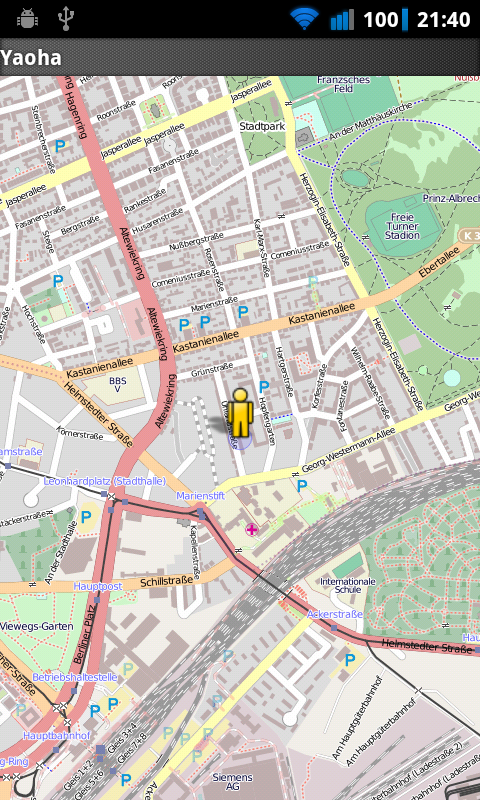
\includegraphics[scale=0.25]{map_plain.png}
  \end{columns}
\end{frame}

\begin{frame}
  \frametitle{Features}
  \begin{columns}
  \column{5.1cm}
    \begin{itemize}
    \item Karten-view
    \alert<1>{\item Darstellen von Geschäften}
    \item (Settings)
    \item View für Suche
    \item Favoriten
    \item Fehlende Öffnungszeiten nachtragen
    \item Daten an OSM übertragen
    \end{itemize}
  \column{5cm}
    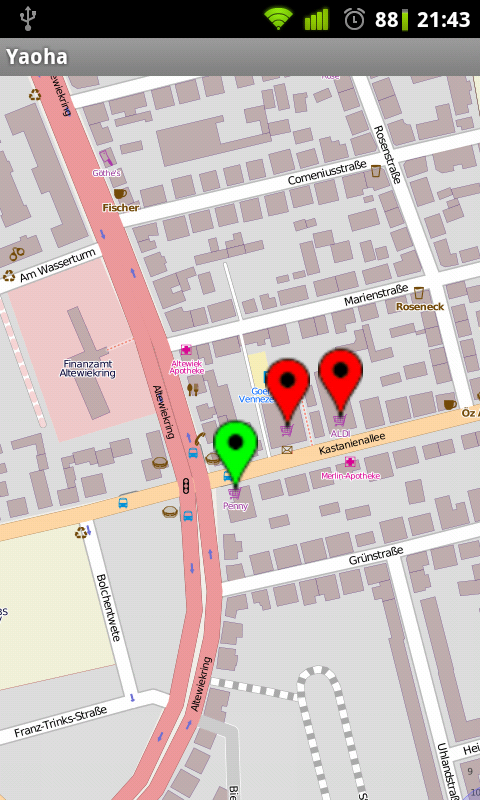
\includegraphics[scale=0.25]{map_shops.png}
  \end{columns}
\end{frame}

\begin{frame}
  \frametitle{Features}
  \begin{columns}
  \column{5.1cm}
    \begin{itemize}
    \item Karten-view
    \item Darstellen von Geschäften
    \alert<1>{\item (Settings)}
    \item View für Suche
    \item Favoriten
    \item Fehlende Öffnungszeiten nachtragen
    \item Daten an OSM übertragen
    \end{itemize}
  \column{5cm}
    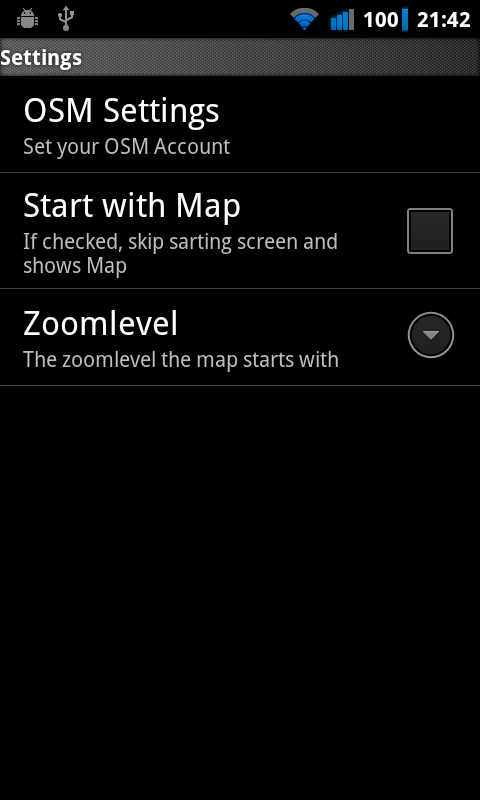
\includegraphics[scale=0.25]{settings1.png}
  \end{columns}
\end{frame}

\begin{frame}
  \frametitle{Features}
  \begin{columns}
  \column{5.1cm}
    \begin{itemize}
    \item Karten-view
    \item Darstellen von Geschäften
    \item (Settings)
	\alert<1>{\item View für Suche}
    \item Favoriten
    \item Fehlende Öffnungszeiten nachtragen
    \item Daten an OSM übertragen
    \end{itemize}
  \column{5cm}
    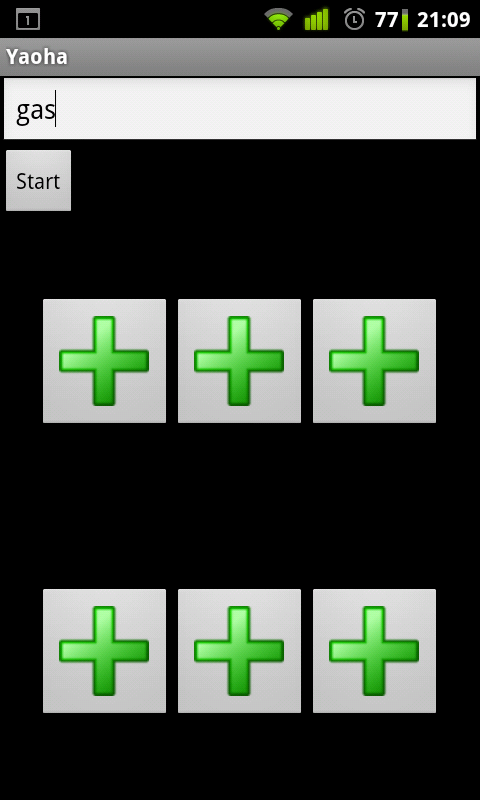
\includegraphics[scale=0.25]{search.png}
  \end{columns}
\end{frame}


\begin{frame}
  \frametitle{Features}
  \begin{columns}
  \column{5.1cm}
    \begin{itemize}
    \item Karten-view
    \item Darstellen von Geschäften
    \item (Settings)
	\item View für Suche
    \alert<1>{\item Favoriten}
    \item Fehlende Öffnungszeiten nachtragen
    \item Daten an OSM übertragen
    \end{itemize}
  \column{5cm}
    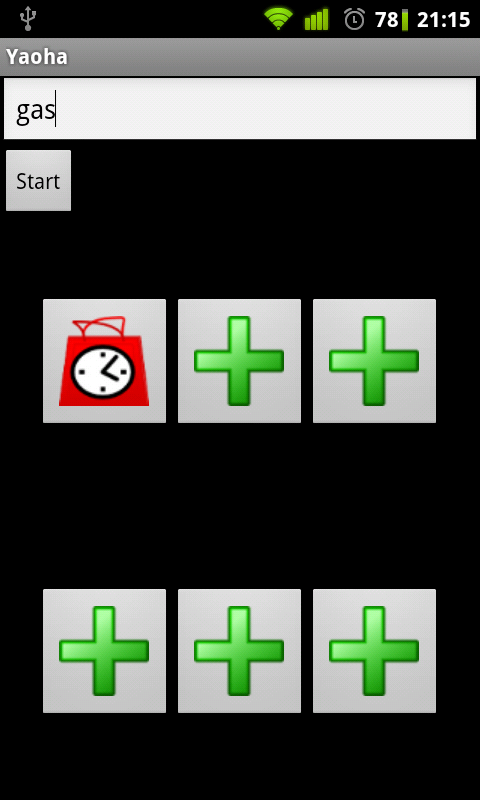
\includegraphics[scale=0.25]{fav2.png}
  \end{columns}
\end{frame}


\begin{frame}
  \frametitle{Features}
  \begin{columns}
  \column{5.1cm}
    \begin{itemize}
    \item Karten-view
    \item Darstellen von Geschäften
    \item (Settings)
	\item View für Suche
    \item Favoriten
    \alert<1>{\item Fehlende Öffnungszeiten nachtragen}
    \item Daten an OSM übertragen
    \end{itemize}
  \column{5cm}
    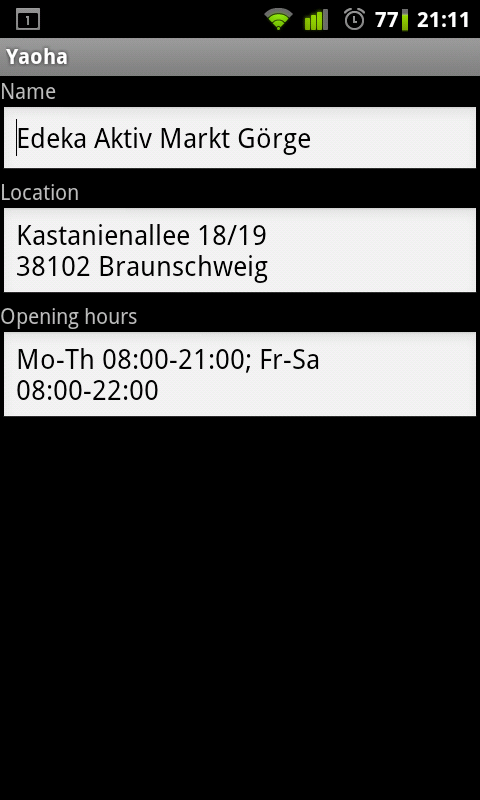
\includegraphics[scale=0.25]{info-panel.png}
  \end{columns}
\end{frame}


\begin{frame}
  \frametitle{Features}
  \begin{columns}
  \column{5.1cm}
    \begin{itemize}
    \item Karten-view
    \item Darstellen von Geschäften
    \item (Settings)
	\item View für Suche
    \item Favoriten
    \item Fehlende Öffnungszeiten nachtragen
    \alert<1>{\item Daten an OSM übertragen}
    \end{itemize}
  \column{5cm}
    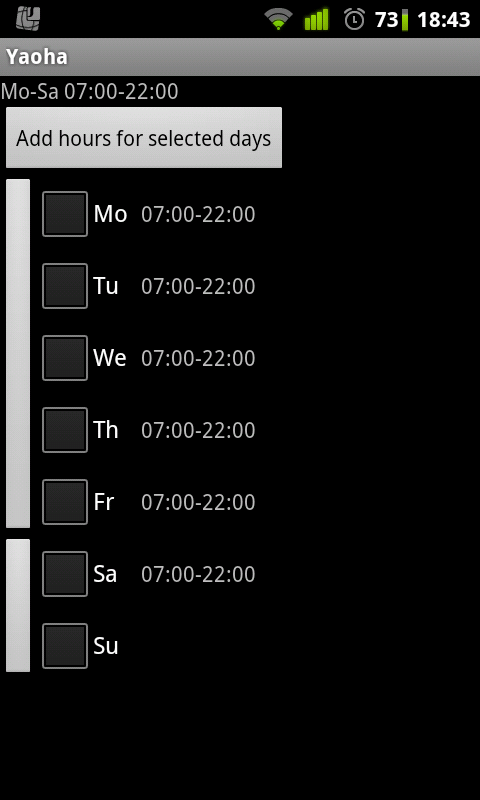
\includegraphics[scale=0.25]{send_opening_hours.png}
  \end{columns}
\end{frame}


\section{Designentscheidungen}
\setbeamercolor{frametitle}{fg=white,bg=tu-red}
\frame{\frametitle{Outline} \tableofcontents[currentsection]}
\setbeamercolor{frametitle}{fg=black,bg=tu-grey}

\begin{frame}{View-Layout}
	\center{Favoriten oder Kartenansicht?}
	\bigbreak
	\begin{columns}
		\column{4cm}	    
	    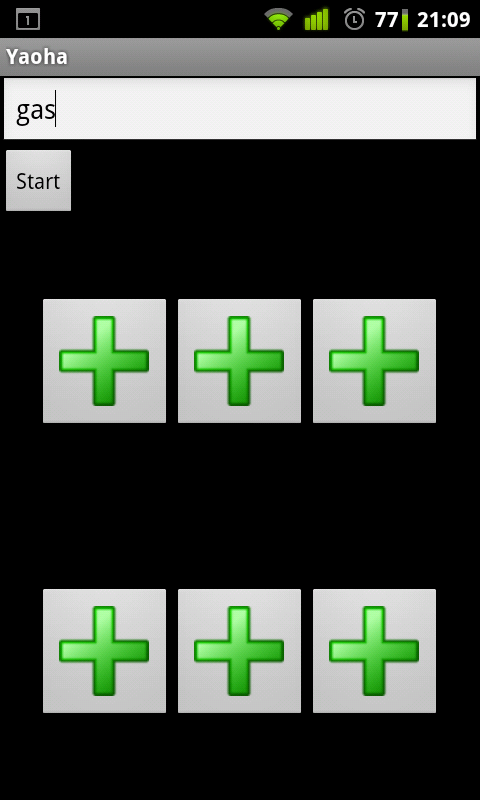
\includegraphics[scale=0.17]{search.png}
	    \column{3cm}
    	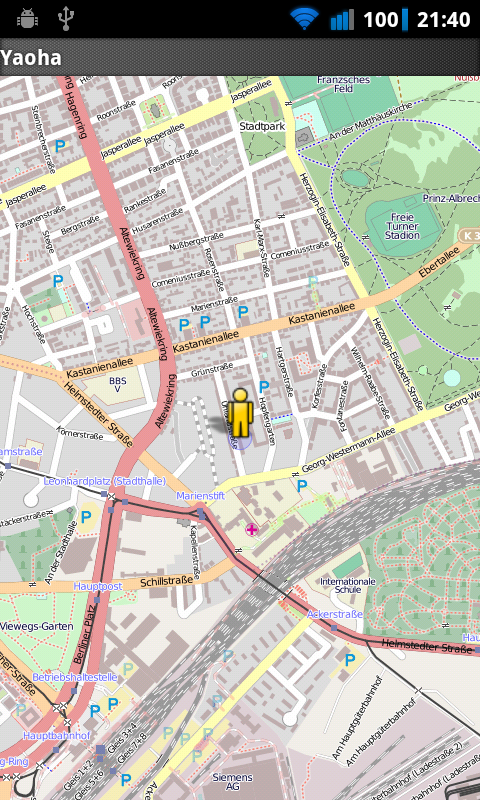
\includegraphics[scale=0.17]{map_plain.png}
    \end{columns}
\end{frame}


\begin{frame}{\"Offnungszeiten}
	\begin{columns}
		\column{5.1cm}	    
		\center{Wie implementieren wir dies am besten?}
	    \column{5cm}
    	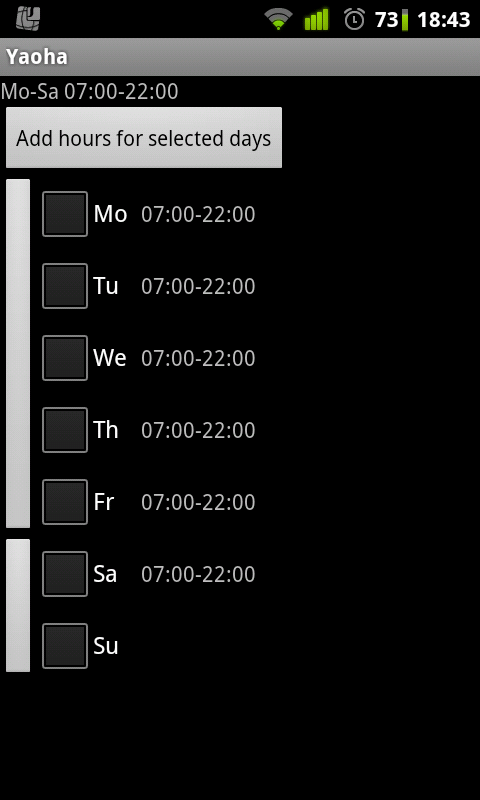
\includegraphics[scale=0.25]{send_opening_hours.png}
    \end{columns}
\end{frame}




\section{Probleme}
\setbeamercolor{frametitle}{fg=white,bg=tu-red}
\frame{\frametitle{Outline} \tableofcontents[currentsection]}
\setbeamercolor{frametitle}{fg=black,bg=tu-grey}


\begin{frame}{Technische Probleme}
	\begin{itemize}
		\item Lokalisation nicht im Emulator testbar (Absturz)
        \item osmdroid MapView API weicht teilweise ab von der Google MapView API
		\item OSM-Öffnungszeiten sind schwierig zu parsen, da
		\begin{enumerate}
		  \item die Syntax sehr umfangreich ist und
		  \item die OSM-Nutzer sich nicht immer an die Syntax halten\\
		  \vspace*{0.1cm}
		  \mbox{z.B. ``Mo 08:00-12:00, 14:00-18:00'' statt ``Mo 08:00-12:00,14:00-18:00''}\\
		  \mbox{z.B. ``Sa 06:00'' statt ``Sa 06:00-11:00'' oder ``Sa 06:00+''}
		\end{enumerate}

	\end{itemize}
\end{frame}


\begin{frame}{Organisatorische Probleme}
	keine, dank...
	\begin{itemize}
		\item Git
		\item Github-Issues
	\end{itemize}
\end{frame}

\section{Ende}
\begin{frame}{Ende}
	\begin{center}
		Danke für eure Aufmerksamkeit!
	\end{center}
\end{frame}

\end{document}
